\chapter{Particle Simulator}
\label{chap:particle-simulator}

The aforementioned many-body systems generally exert very complex behaviour when viewed as a whole.
This behaviour can be captured in mathematical terms but also from a simulation perspective.
Particle simulations have been a subject of much attention in physics and scientific computing more generally.
This class of simulations, in the context of intermolecular interactions, is often referred to as molecular dynamics.

\begin{figure}[H]
  \centering
  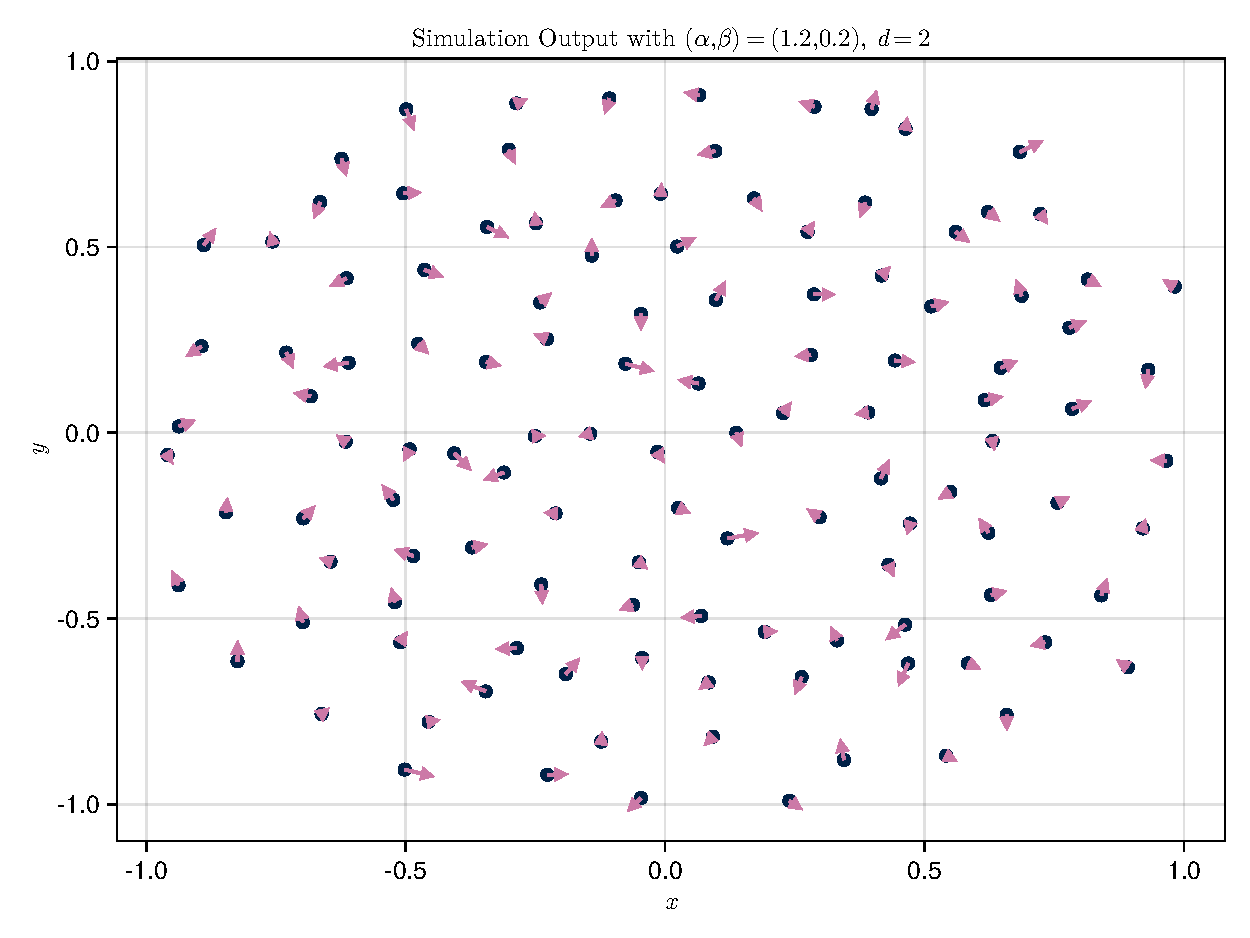
\includegraphics[width=0.8\linewidth]{results/known-2d/simulation-quiver.pdf}
  \caption[Quiver plot of 120 particles in 2D interacting through the attractive-repulsive potential]{Position and velocity of particles in the simulation at a point in time. Every particle, each of equal mass $m$, interacts with every other particle through the interaction potential $U_{ij} = K\left(\norm{\vec{x_i} - \vec{x_j}}\right)$ leading to $\mathcal{O}(N_p^2)$ interactions.}
  \label{fig:simulation-quiver}
\end{figure}

Because each particle interacts with every other particle, the number of interactions scales with $\mathcal{O}(N_p^2)$,
which can play a prohibitive role in terms of the computation time when increasing the number of particles $N_p \gg 1$.

Within the scope of this thesis, in order to understand the elaborate behaviour of such particle systems and also to verify results from theory and the spectral method, we provide an implementation of a simulator starting from a numerical time integrator in $\R^d$.
In addition to the \textit{headless} simulation software, exporting state and results for treatment by the analysis component, a \gls{gui} is provided to enable live insight into and interaction with the model.

\begin{figure}[H]
  \centering
  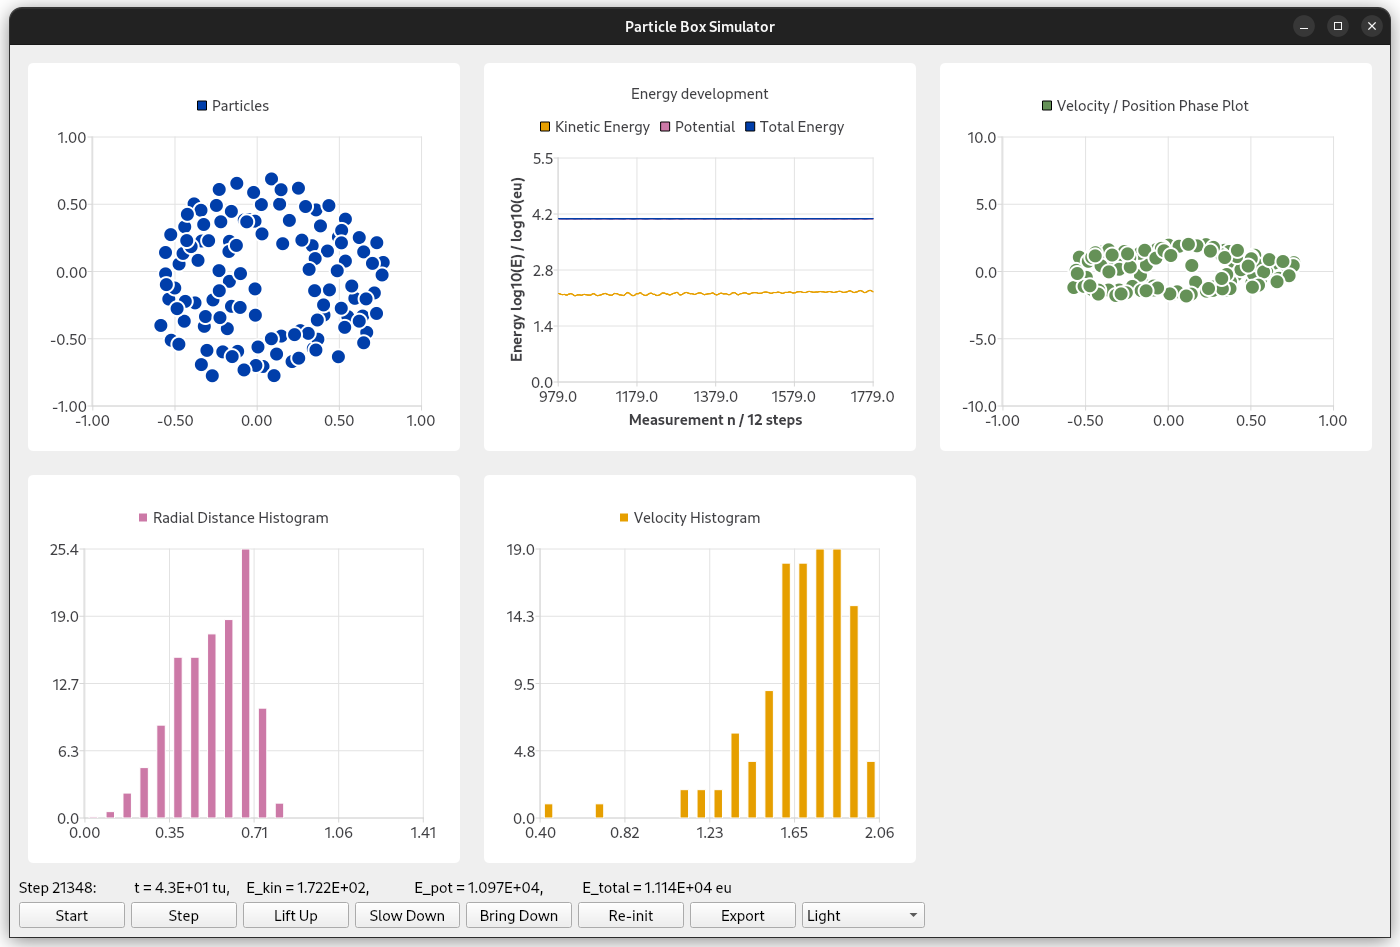
\includegraphics[width=\linewidth]{gui-screenshot.png}
  \caption[Graphical User Interface of the Simulator]{Screenshot of the \gls{gui} provided for the particle simulator. The top row shows the position of particles in their $[-1, 1]^d$ ($d = 2$ in this case) domain at a point $t$ in time, the energy development over time and the current position/velocity phase space plot. Below, there are position and velocity histogram updated live along with the simulation.}
  \label{fig:gui-screenshot}
\end{figure}

\section{Available Methods}
\begin{itemize}
  \item Simple Forward Integration
  \item Multistep Methods, which is an extension to the simple integration above.
  \item Fast Multipole Method
  \item Multigrid Methods
\end{itemize}
\hierKoennteIhreWerbungStehen

\subsection{Leapfrog Integration}
% Nice introduction \href{https://lemesurierb.people.cofc.edu/introduction-to-numerical-methods-and-analysis-julia/docs/ODE-IVP-6-multi-step-methods-leapfrog-julia.html}{here}.
% Maybe compare with \href{https://turinglang.org/AdvancedHMC.jl/stable/}{Advanced HMC}?
\hierKoennteIhreWerbungStehen
% TODO: vielleicht eine kleine Figure zur Visualisierung des Leap-Frogs

% where we note that $\nabla f(\norm{\vec{x}}) = \frac{\vec{x}}{\norm{\vec{x}}} f'(\norm{\vec{x}})$.

\section{Phase Space}
Each particle, at every point in time $t$, has a position and velocity value.
In $d=1$ dimension, one can visualise both of these quantities simultaneously in a phase space plot (cf. \Cref{fig:phase-space-plot}).
For $d > 1$ dimension, it is possible to either only visualise the first components $\{\vec{x_i}\}_1$ and $\{\vec{v_i}\}_1$ or to visualise the norm of the position (distance from the centre of mass) $r = \norm{\vec{x_i} - \vec{x}_{\text{centre}}}$ and velocity $\norm{\vec{v_i}}$, where $$\vec{x}_{\text{centre}} := \frac{1}{N_p} \sum_{i=1}^{N_p} \vec{x_i}\,.$$

\begin{figure}[H]
  \centering
  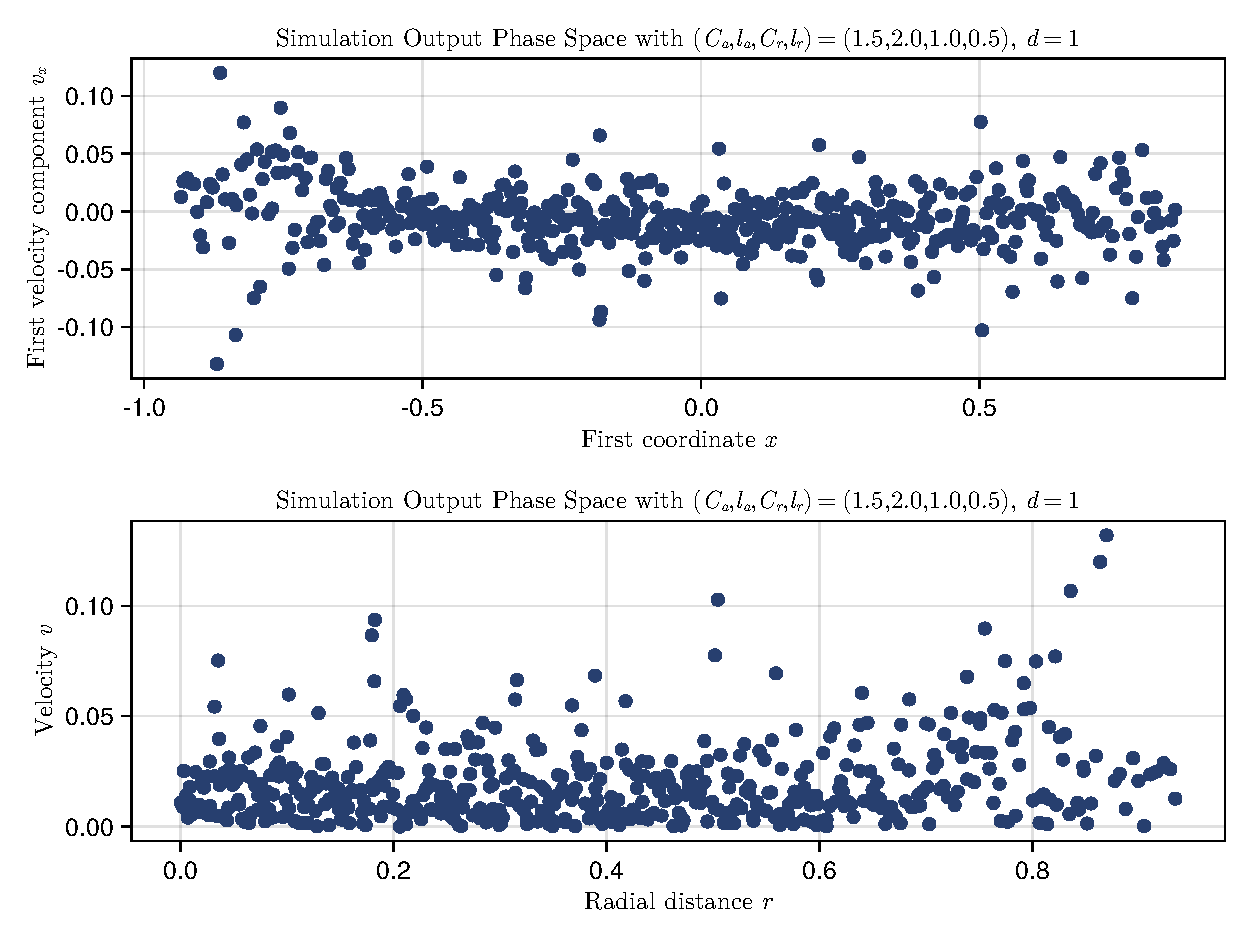
\includegraphics[width=0.8\linewidth]{results/morse/phase-space-plot.pdf}
  \caption[Phase Space Plots]{Position and velocity of $N_p = 500$ particles in a $d=1$ simulation visualised as phase space plots using the two different visualisation mechanisms. In the top plot, one can observe natural rotation around the origin $(0, 0)$ as positive velocity corresponds to movement to the right and negative velocity to leftwards movement.}
  \label{fig:phase-space-plot}
\end{figure}

The behaviour of the phase space plot differs from potential to potential, most importantly one can observe multiple centers of rotation for the Morse potential in addition to the origin, whereas an attractive-repulsive potential builds up to an elliptical shape in the phase space plot.
% TODO: why is this? Local interactions?

\begin{figure}[H]
  \centering
  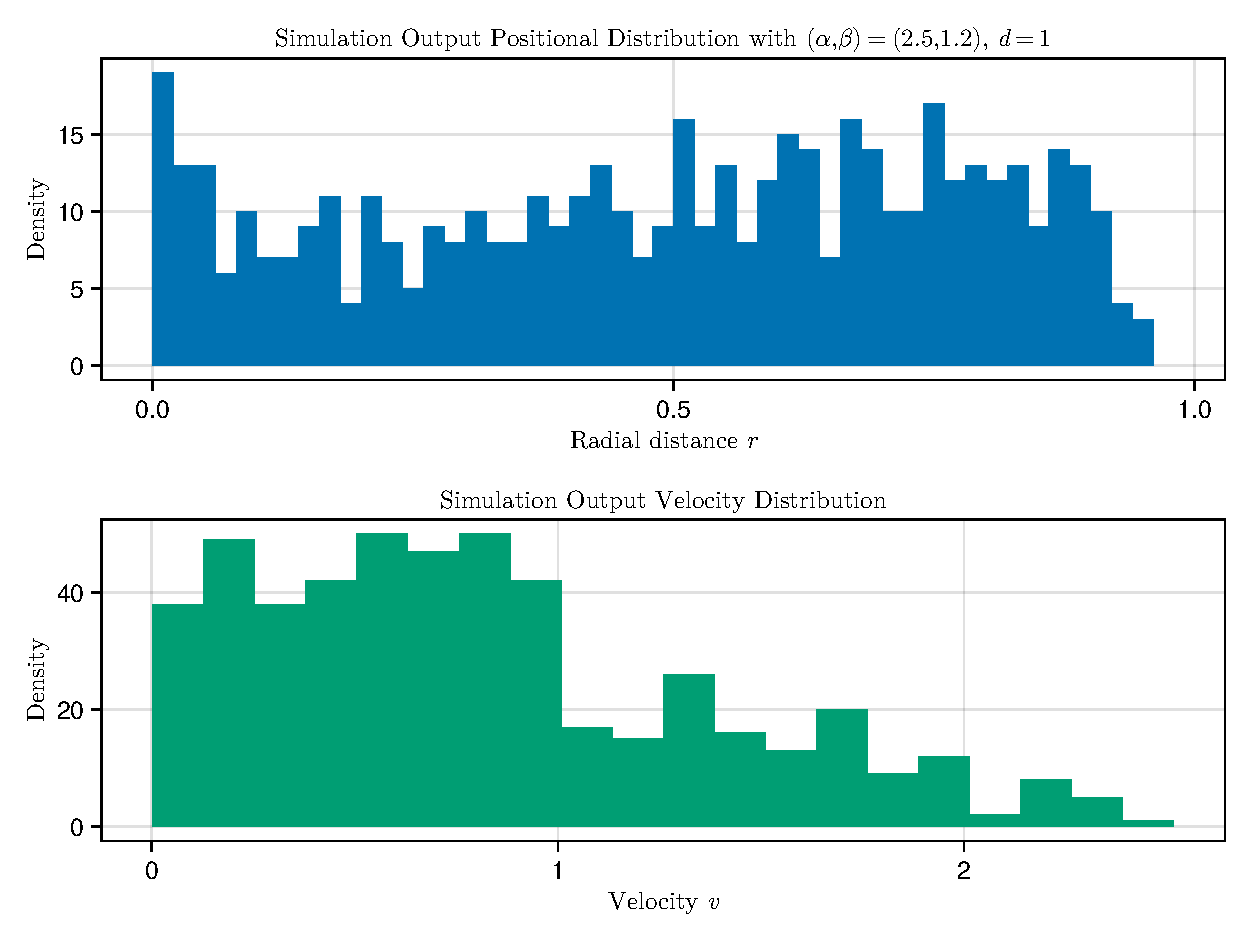
\includegraphics[width=0.8\linewidth]{results/attrep/simulation-histogram.pdf}
  \caption[Radial Distance and Velocity Histograms of attractive-repulsive Simulation Output in 1D]{Radial Distance ($r$) and Velocity ($v$) Histograms as obtained through a long-running simulation of $N_p = 500$ particles interacting through an attractive-repulsive potential $K_{\alpha, \beta}(r)$. The spectral method introduced in \Cref{chap:spectral-method} aims to solve for the particle density as a function of radial distance, hoping to predict the shape of the positional histogram.}
  \label{fig:simulation-histogram}
\end{figure}

In a physical setting with collision terms, the velocity distribution $f(v)$ would approach the shape of a Boltzmann distribution
$$f(v)={\bigg(\frac{m}{2\pi k_B T}\bigg)}^{\frac {3}{2}}\,4\pi v^{2}\exp \left(-{\frac {mv^{2}}{2k_B T}}\right)\,,$$
where $k_B$ is the Boltzmann constant and $T$ is temperature.

\section{Runtime Analysis}
\hierKoennteIhreWerbungStehen
